\documentclass[12pt, oneside]{article}   	% use "amsart" instead of "article" for AMSLaTeX format
\usepackage{textcomp}
\usepackage{geometry}                		% See geometry.pdf to learn the layout options. There are lots.
\geometry{letterpaper}                   		% ... or a4paper or a5paper or ... 
%\geometry{landscape}                		% Activate for rotated page geometry
%\usepackage[parfill]{parskip}    		% Activate to begin paragraphs with an empty line rather than an indent
\usepackage{graphicx}				% Use pdf, png, jpg, or eps§ with pdflatex; use eps in DVI mode
\usepackage{caption}
\usepackage{subcaption}								% TeX will automatically convert eps --> pdf in pdflatex		
\usepackage{hyperref}
\usepackage{amssymb}
\usepackage{amsthm}
\newtheorem{theorem}{Theorem}
\newtheorem{definition}{Definition}
\usepackage{natbib}
\usepackage{xcolor}
\usepackage{hyperref}
\usepackage{authblk}
\hypersetup{
    colorlinks=false,
    linkcolor=blue,
    filecolor=magenta,      
    urlcolor=blue,
    pdfpagemode=FullScreen,
}
\usepackage{float}
\usepackage{rotating}
\usepackage{adjustbox}
\usepackage[font=small,labelfont=bf]{caption}

\usepackage{authblk}
\title{Detecting Overlapping Research Communities}
\author[1]{Akhil Jakatdar}
\author[1]{Tandy Warnow\thanks{warnow@illinois.edu}}
\author[1,2]{George Chacko\thanks{chackoge@illinois.edu}}
\affil[1]{Department of Computer Science, University of Illinois Urbana-Champaign, Urbana, IL 61801}
\affil[2]{Office of Research, Grainger College of Engineering, University of Illinois Urbana-Champaign, Urbana, IL 61801}

% \setlength{\parindent}{0pt}
%SetFonts

\begin{document}
\maketitle

\abstract{[\emph{Rewrite after the rest of the paper is completed.} Community detection assists the understanding of complex networks and a variety of clustering methods have been developed for this purpose. Unsurprisingly, a rich literature exists, originating from several fields, on developing and applying community detection. However, many community finding methods rely on disjoint clustering in which a node is only assigned to one community or cluster. This strict requirement limits the ability to inclusively describe communities since some nodes may reasonably be assigned to many communities. Whereas, we previously described a scalable and modular pipeline that discovers disjoint communities, we now present a complementary overlapping community approach.  We report findings from this new approach on a network of over 13 million nodes that captures recent research in the very rapidly growing field of extracellular vesicles in biology. We wanly declare relief at not having studied Zachary's Karate Club.}

\clearpage

\section{Introduction} Research communities represent scientific specialization \citep{Chubin1976,Morris2009} that evolves in response to influences such as new research paradigms, policy effects, collaboration practices, increasing globalization, and large-scale reorganization.The work presented in this article is motivated by the problem of identifying and characterizing research communities in the modern scientific enterprise.  We are interested in scalable methods for identifying research communities as they emerge and grow to maturity, and would like to understand the extent to which these communities overlap. 

An approach to identifying research communities is through analyzing citation patterns in the scientific literature. The underlying assumption is that members of a research community are more likely to cite each other's work than the work from outside their community.  Drawing upon the rich literature on graph theory, this question can then be framed as a community finding problem where a community is defined as a set of vertices in a graph that exhibit stronger connectivity to each other than to vertices outside such a community. Thus, in the graph (or network) of scientific literature, citation-dense areas suggest the existence of communities of publications. Finally, the authors extracted from a community of publications are assumed to form a research community \citep{Chandrasekharan2021,Wedell2022}. This community discovery approach is similar to constructing article level clusters \citep{Waltman2012,Traag2019} and is the inverse of characterizing the publications authored by members of defined known communities \citep{Price1966,crane1972invisible,smallspecialties1979,Mullins1985}. 

We stress that citation density alone does not make a confirming argument for the existence of a community. However, community finding techniques are valuable in being able to efficiently search large datasets for communities that can then be examined with complementary techniques, ideally supported by domain expertise.

Beyond community detection, however, we are also interested in substructure (specifically, structure within communities), as it reflects roles and dynamics among members. \cite{Price1966}, in their study of the oxidative phosphorylation community, reported center-periphery substructure \citep{Breiger2014}: a small core of influential researchers and a much larger transient population. Core-periphery or center-periphery patterns have also been reported in other networks using different techniques, such as block modeling and k-core decomposition arguing for some degree of ubiquity in their occurrence \citep{borgatti2000models,Rombach2017,gallagher2021clarified,yanchenko_2202.04455}. 

A considerable literature exists on community finding in graphs, and a variety of community finding or clustering approaches have been used in scientometrics~\citep{Newman2006,Fortunato2009,Boyack2010,Boyack2019,Traag2019,Ahlgren2020,Chandrasekharan2021,Wedell2022}. The majority of these approaches focus on disjoint partitioning, where a vertex is only assigned to one community. 

We recently reported Iterative K-core Clustering or IKC \citep{Wedell2022}, a recursive algorithmic approach based on the k-core property \citep{Giatsidis2011,malliaros2019}, which helps identify densely connected parts of a graph. IKC recursively extracts disjoint k-cores from a graph beginning with the most dense  k-core and until some user-specified value of $k$ is reached. 

We implemented IKC as the first step in a tunable modular pipeline to identify communities with core-periphery structure. Subsequent steps in the pipeline include breaking large cores, and adding peripheral nodes to each core to construct communities with core-periphery structure. We applied this pipeline to a network of roughly 14 million articles rooted in the rapidly growing field of extracellular vesicle biology \citep{Wedell2022}. 

A limitation of IKC is that  it produces disjoint clusters, and some articles can reasonably be assigned to more than one community. This limitation is especially relevant to articles that describe widely used methods but is conceivably also relevant to articles reporting discovery that are influential in more than one community.   However, this is a problem with nearly all clustering methods, and suggests a need for methods that can produce meaningful overlapping clusters. 

Several methods have been developed that can produce overlapping clusters although none of them were designed to specifically address core-periphery structure in the scientific literature  \citep{Baumes2005,Palla2005,banerjee2005model,Cleuziou2008,Lancichinetti2009,Lu2012}. Another approach uses a two-step procedure where the input graph is first transformed into a line graph whose nodes represent edges in the original graph \citep{Harary1960}.  The line graph is then clustered and this output can be mapped back to the input graph to generate overlapping clusters. This general approach has been used by others on citation data \citep{Evans2009,Havemann2021}. However, line graph  techniques are not very scalable, since the size of a line graph is much larger than the size of its input graph. For example, the network that we studied in \cite{Wedell2022} would grow from 13,989,436 nodes and 92,051,051 edges to 92,051,051 nodes and 160,428,881,121 edges (Supplementary Materials), which presents a challenge to clustering software.
 
To address the disjoint cluster problem with IKC, we present ``Allowing Overlapping Clusters" (AOC), a scalable meta-method that takes the output of IKC and makes multiple community assignments from a list of candidate nodes. We present results from AOC applied to the cores generated by the IKC method, and discuss the results and discovery made from them.
 
\section{Materials and Methods}

\subsection{Data} 

\emph{Citation network} We previously generated a citation network \citep{Wedell2022} representing the exosome \citep{harding1983} and more generally the extracellular vesicle literature \citep{raposo2021}. The network from the Dimensions database \citep{hook2018dimensions} in the Google cloud. For the present study, we curated this network to deplete it of both retracted articles and relatively high-referencing articles. Retractions, were identified from a database kindly provided by Retraction Watch and matched to nodes in the network using digital object identifiers (DOIs). Any article with 250 or more references was also removed. Whereas the original network consisted of 14,695,475 nodes and 99,663,372 edges, the network resultant from removing retracted and high-referencing articles comprised 13,989,436 nodes and 92,051,051 edges; we refer to this network as   the Curated Exosome Network (CEN). Its largest connected component consists of 13,988,426 nodes and accounts for 99.99\% of the CEN.

\emph{Marker nodes}. To identify exosome-relevant publications and communities, we re-used a set of marker nodes described in  \citep{Wedell2022}. These 1218 markers are the cited references combined from 12 different recent review articles on exosomes and extracellular vesicles. Of these, 1021 are present in the CEN. 

\subsection{Methods} Motivated by the graph-theoretic concept of k-cores \citep{Giatsidis2011,malliaros2019}, we have previously constructed a clustering pipeline we refer to as  the Iterative K-core Clustering (IKC) pipeline in \cite{Wedell2022}, This scalable and tunable method takes, as input, two parameters $k$ and $p$ with $k > p \geq 1$, and computes a clustering of a given network $N$ into disjoint clusters where each cluster has a ``core'' component, and a ``periphery". This clustering is designed to satisfy several criteria: (1) the core of each cluster is connected,  has positive modularity ($m$-valid), and each node in the center  is adjacent to at least $k$ other nodes in the center ($k$-valid), and (ii) every node in the periphery of a cluster is adjacent to at least $p$ center nodes in the cluster ($p$-valid). Thus, membership of the core of a cluster requires a greater degree of connectivity to the other center nodes than membership of the periphery. 

The IKC pipeline has three basic steps, where the second and third steps are optional.  The first step (the iterative k-core extraction algorithm) produces disjoint $km$-valid clusters where each cluster has positive modularity and each node in each cluster is adjacent to at least $k$ other nodes in the cluster; these form the centers or cores of the communities. The optional second step breaks these clusters into smaller clusters, and the optional third step adds peripheries to the clusters.  Note that the parameter $k$ is used to define the centers and the parameter $p$ is used to define the periphery. If the only objective is cores or centers of communities, then the pipeline can be run using only the first step (or optionally also with the second step if smaller communities are desired).

The Allowing Overlapping Clusters (AOC) method, presented herein, builds on the first step of the IKC pipeline (k-core extraction). To run AOC, the user specifies two additional parameters:  
the set of nodes that can be members of  additional clusters and the criterion for membership.  The two criteria for membership in the core of cluster $C$ we consider are: (i) to have at least $k$ neighbors 
in the core of $C$ or (ii) to have at least $MCD(C)$ neighbors in the center of $C$, where $MCD(C)$ is the minimum core degree; the minimum number of center neighbors of any node within $C$. 
We note that $k$ (the parameter for condition (i)) has been used to construct the IKC clustering; hence, for every cluster $C$,  (i) is a weaker condition than (ii).
We refer to the first as AOC\_k and the second as AOC\_m.

Thus, running   AOC on the IKC clustering produces a set of potentially overlapping clusters, each of which has positive modularity and has at least $k$ other nodes in the cluster. These clusters form the cores of communities.  This study is focused on core structure but the clustering process could be extended to the same optional second and third steps from the IKC pipeline, which would break up the large clusters and add peripheral nodes. 

\section{Results and Discussion}

As we explain in the preceding sections, AOC is a meta-method for overlapping communities that takes as input, a k-core based clustering such as IKC, a set of candidate nodes for consideration of membership in multiple communities, and a parameter that defines the criterion for membership. We now examine the properties of non-disjoint clusterings produced using IKC and AOC in tandem. 

\subsection{Experiment 1: Comparison to random networks} In an initial calibration experiment, we clustered the curated exosome network (CEN) using IKC where $k \in {\{10,20,30,40, 50\}}$. The resultant distribution of cores is consistent with our observations in \cite[Figure~3]{Wedell2022}, with maximum coverage seen at the lowest value of $k$ used. At the value of $k$ with maximum coverage (IKC\_k10), 128 $km$-valid cores, containing a total of 535,165 nodes (0.54\% of the CEN network) are discovered. These cores range in size from 14 to 214,877, with a median core size of 79, and minimum core degree (MCD) varying from 10-53 with median MCD of 16. Thus, the CEN is a 53-degenerate graph consisting of 13,989,436 vertices.

To examine random network effects that could contribute to observed results from IKC, we generated 10 replicates of a configuration null model where the edges of the input clustering were randomized while preserving the total number of nodes, the degree of each node, the total number of nodes, and the publication year of each cited node in a citing-cited node pair. These shuffled networks were then clustered using IKC with  $k=10$ (IKC\_k10). In all 10 cases, only a single $km$-valid core with MCD of 15 was extracted, although the number of nodes in each of these cores varied as did modularity of the core (Table~\ref{tab:tab1}). The median size of this cluster across 10 replicates was 435,216. We did not run IKC at higher values for $k$ on the random networks since  the minimum core degree (MCD) of 15 for the single cluster would have been exceeded and not result in any clusters. 

We also generated 100 replicates of an Erd\H{o}s-Renyi graph with the same number of nodes and edges as the CEN network and clustered them with IKC\_k10 (Supplementary Material). No $km$-valid clusters were generated from the Erd\H{o}s-Renyi graphs. Thus, the results seen in IKC clustering on a real world network are unlikely to be the result of random effects. We did not run AOC on the IKC output from either the configuration models or the Erd\H{o}s-Renyi graphs since it would not have any effect on a on a single cluster or no clusters.

. 
% derived from k_10_totaldegree_1percent_original_cluster_stats.csv in /shared/aj_manuscript_data/experiment_1/. 

% > shuffled_df
%   cluster_no   mcd modularity node_count                cluster_id
%         <int> <int>      <num>      <int>                    <char>
% 1:          1    15 0.01110796     435216  shuffled_ikc1.clustering
% 2:          1    15 0.01094716     425275 shuffled_ikc10.clustering
% 3:          1    15 0.01119657     443254  shuffled_ikc2.clustering
% 4:          1    15 0.01125269     440106  shuffled_ikc3.clustering
% 5:          1    15 0.01132720     448858  shuffled_ikc4.clustering
% 6:          1    15 0.01126005     432842  shuffled_ikc5.clustering
% 7:          1    15 0.01131381     446305  shuffled_ikc6.clustering
% 8:          1    15 0.01122132     436192  shuffled_ikc7.clustering
% 9:          1    15 0.01106562     424074  shuffled_ikc8.clustering
%10:         1    15 0.01105279     436273 shuffled_ikc9.clustering

\begin{table}[ht]
% data drawn from xtable product above using
% collate_shuffled_results.R gc 7/3/2022
\centering
\captionsetup{width=0.9\textwidth}
\caption{IKC clustering of Configuration Null Model. The edges of the CEN network were randomly redirected while preserving degree distribution for each node and the year of publication for citing and cited nodes. 
The resultant network was clustered with IKC with k=10.  In all 10 cases, a single k-core with minimum core degree of 15 resulted although the size and modularity of these cores vary. In contrast, the IKC(10) analysis of the original CEN (unperturbed) network produced 128 cores  with minimum core degrees ranging from 10 to 52.}
\begin{tabular}{lcccc}
  \hline
cluster\_id & cluster\_no & mcd & modularity & node\_count  \\ 
  \hline
shuffled\_CEN\_network-1 &     1 &    15 & 0.0111 & 435,216 \\
shuffled\_CEN\_network-2 &     1 &    15 & 0.0109 & 425,275 \\
shuffled\_CEN\_network-3 &     1 &    15 & 0.0112 & 443,254 \\
shuffled\_CEN\_network-4 &     1 &    15 & 0.0113 & 440,106 \\
shuffled\_CEN\_network-5 &     1 &    15 & 0.0113 & 448,858 \\
shuffled\_CEN\_network-6 &     1 &    15 & 0.0113 & 432,842 \\
shuffled\_CEN\_network-7 &     1 &    15 & 0.0113 & 446,305 \\
shuffled\_CEN\_network-8 &     1 &    15 & 0.0112 & 436,192 \\
shuffled\_CEN\_network-9 &     1 &    15 & 0.0111 & 424,074 \\
shuffled\_CEN\_network-10 &    1 &   15 & 0.0111 & 436,273 \\ 
   \hline
\end{tabular}
\label{tab:tab1}
\end{table}


\subsection{Experiment 2: Effect of AOC on IKC clusters} 
As previously noted, a limitation of disjoint clustering methods is that restricting membership to one community, excludes assignment to other communities where a node may have both role and influence. Since clustering with IKC occurs recursively, nodes in an extracted core are not considered for membership as other cores are extracted. 

Accordingly, we asked whether AOC could redistribute nodes from disjoint cores generated by IKC to other cores in the same clustering. 
In this experiment, the input clustering was produced by IKC with the CEN network as input and $k \in \{10, 20, 30, 40, 50\}$; the set of candidate nodes was every node within the cores generated by IKC; and the criterion for membership was either (i) AOC\_m or AOC\_k (defined above).

By construction, the number of cores cannot change by running AOC  under any setting of its algorithmic parameters. However, core sizes can increase, with increases resulting from AOC\_k being at least as large as increases resulting from AOC\_m.
Of interest, therefore, is how the algorithmic parameter, such as the value for $k$ and the specified subset of nodes, impact the increase in size, and how node properties, such as degree, influence the number of clusters they are added to.

Figure~\ref{fig:fig1} shows the distribution of cluster sizes generated by AOC relative to the core sizes from the IKC run at various values for \emph{k}. For both AOC\_m and AOC\_k a subset of the clusters increases in size (Table~\ref{tab:tab1} ).
Approximately 74\% and 87\% of  128 cores increase in size with AOC\_m and AOC\_k treatment respectively when IKC with k-10 is used as the input clustering. AOC treatment of IKC clustering, therefore, results in an increase in cluster sizes that is is inversely related to the value of \emph{k} used in IKC and is more pronounced with AOC\_k than with AOC\_m. 

\begin{figure}[H]
\centering
	\begin{subfigure}[t]{0.48\textwidth}
	 \centering
	 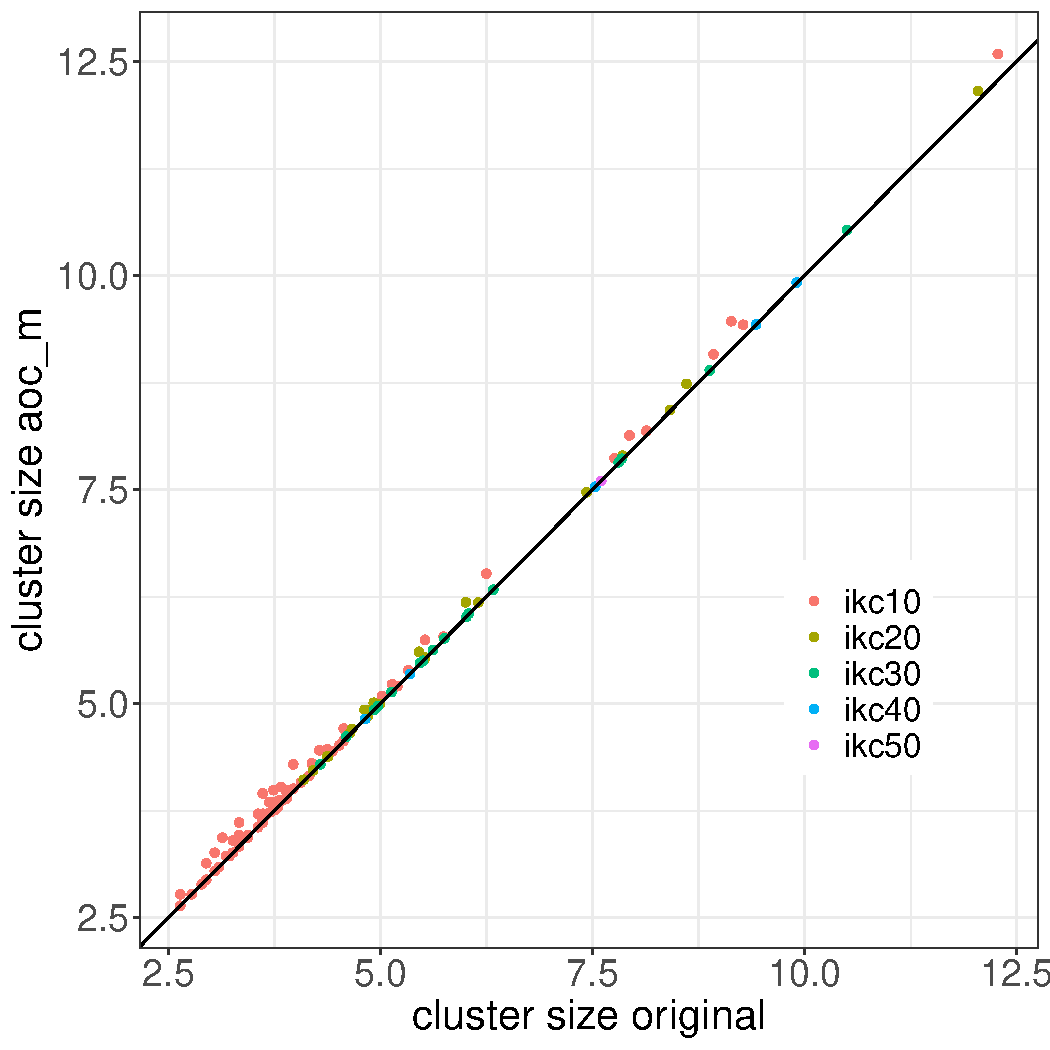
\includegraphics[width=\linewidth]{fig1b.pdf} 
	 \end{subfigure}
 \hfill
	\begin{subfigure}[t]{0.48\textwidth}
        \centering
        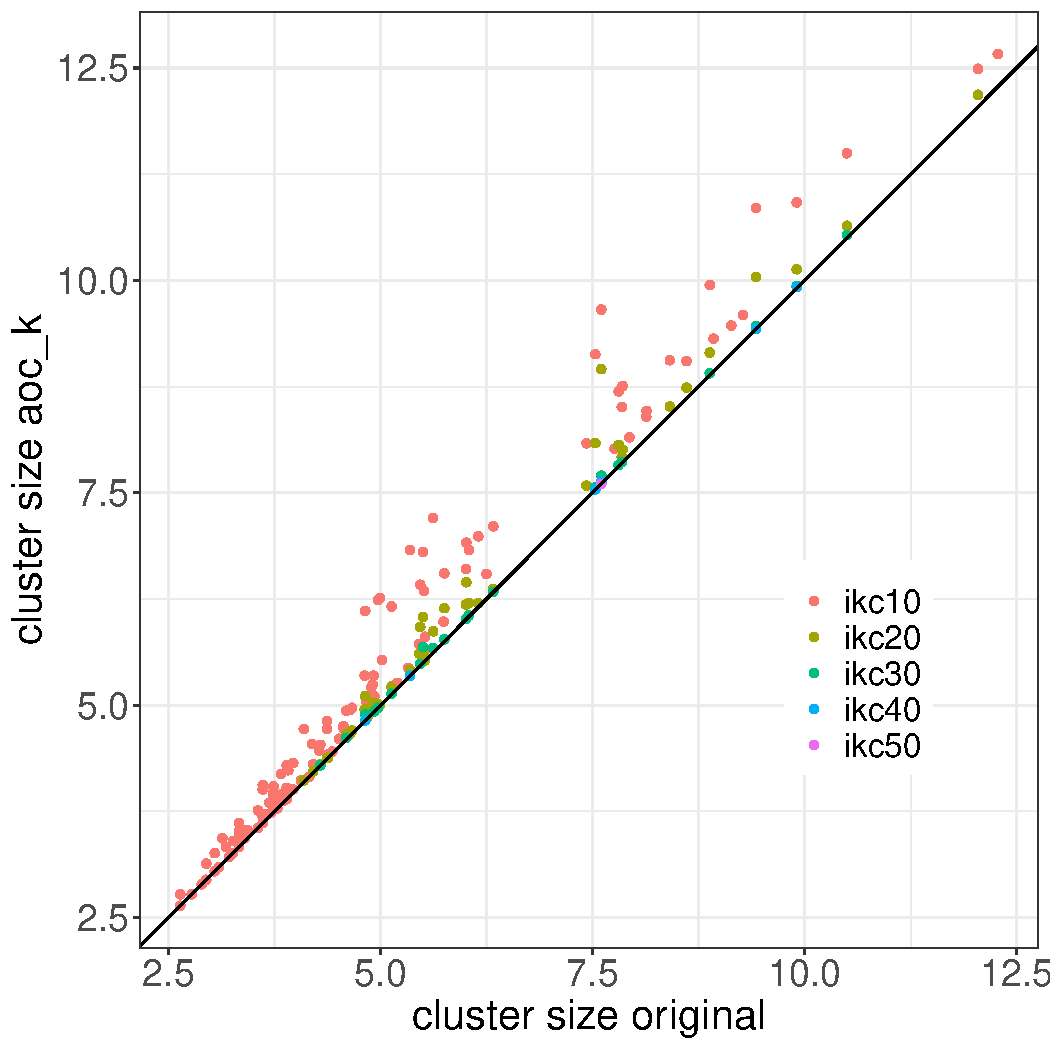
\includegraphics[width=\linewidth]{fig1a.pdf} 
        	\end{subfigure}
\captionsetup{width=0.9\textwidth}	
\caption{Comparison of cluster sizes between disjoint (IKC)  and overlapping (AOC) clusters. Clusters were generated from the CEN network by IKC using values of $k$ ranging from 10 to 50. These clusters were then enriched through the AOC process enforcing either \emph{mcd} (left panel) or \emph{k} (right panel). The input to AOC was the  clustering produced by 
IKC, the value $k$ used to construct the clustering, and the set of nodes to be distributed to additional clusters was all the nodes in the IKC clusters.  Points that lie on the diagonal indicate no change in cluster size after AOC treatment. A natural log scale is used for both axes.}
\label{fig:fig1}
\end{figure}

We then examined the distribution of clusters per candidate node after AOC treatment of clusterings generated by  IKC with $k \in \{10, 20, 30, 40, 50\}$. For AOC\_k treatment of IKC\_k10 clusters, 54\% nodes were assigned to between 2 and 24 clusters in a progressively decreasing manner with roughly 26\% of nodes assigned to 2 clusters and a single node being assigned to 24 different clusters (Table~\ref{tab:tab2}). The remaining 46\% of the nodes were assigned to a single cluster. AOC\_m in comparison to AOC\_k, results in fewer multiple cluster assignments because of its more stringent membership criterion (Table~\ref{tab:tab2} and Figure~\ref{fig:fig2}).

\begin{figure}[H]
	\centering
	\begin{subfigure}[t]{0.48\textwidth}
	 \centering
	 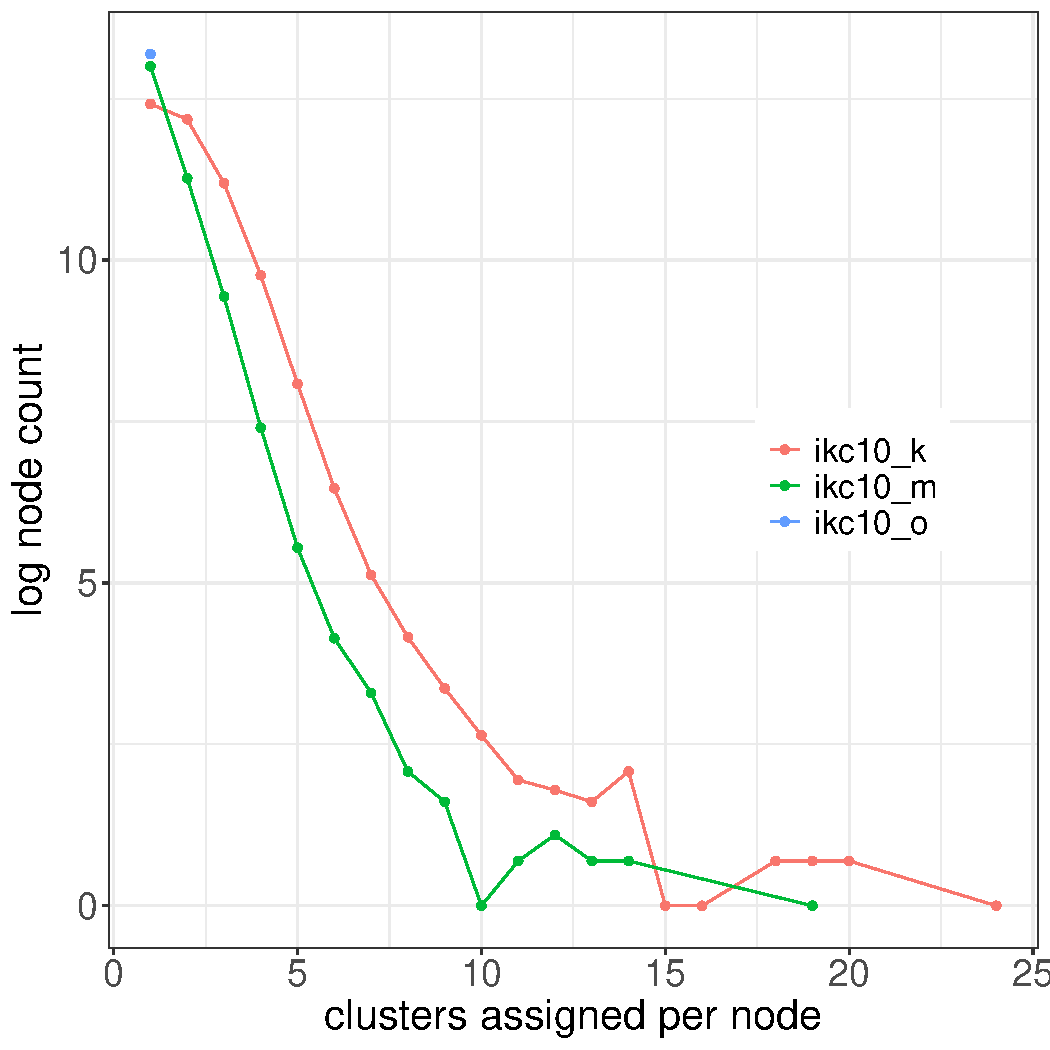
\includegraphics[width=\linewidth]{fig2a.pdf} 
	 \end{subfigure}
 \hfill
	\begin{subfigure}[t]{0.48\textwidth}
        \centering
        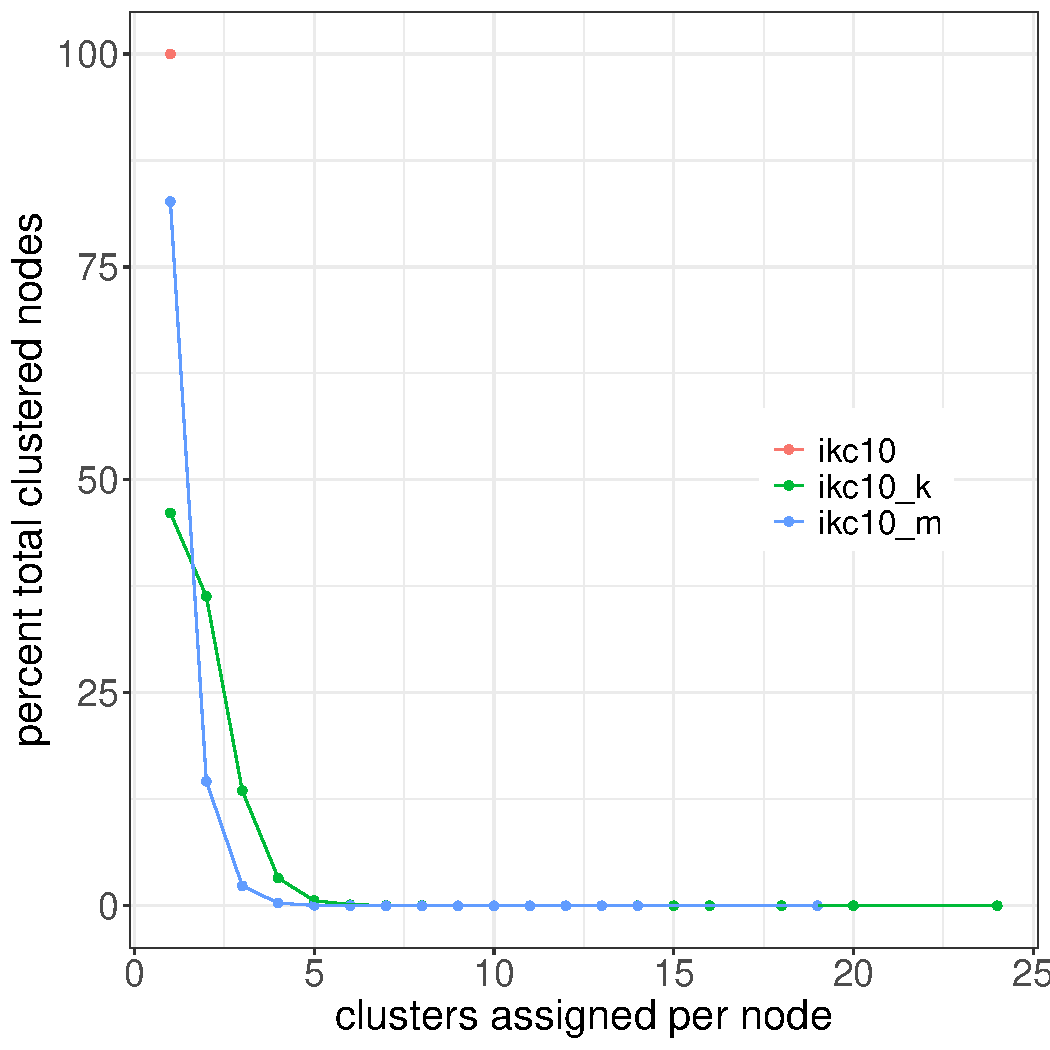
\includegraphics[width=\linewidth]{fig2b.pdf} 
    	\end{subfigure}
\captionsetup{width=0.9\textwidth}	
\caption{AOC selectively assigns nodes to multiple clusters. The figure shows the count of nodes (abscissa) grouped by how many clusters a node was assigned to after AOC treatment enforcing either \emph{k} (red) or \emph{mcd} (green);  these are shown as natural log counts (left panel) or percentages of the number of nodes (right panel) in non-singleton clusters. A single node is assigned to 24 different clusters in teh case of AOC\_k. The single blue point in both plots indicates that all the nodes in the input IKC\_k10 clustering are in single clusters.}
\label{fig:fig2}
\end{figure}

\subsection{Experiment 3: Which node properties impact multiple assignments?}

\begin{figure}[H]
% generated by fig_tier_cluster_counts_3.R 
\centering
	\begin{subfigure}[t]{0.48\textwidth}
	 \centering
	 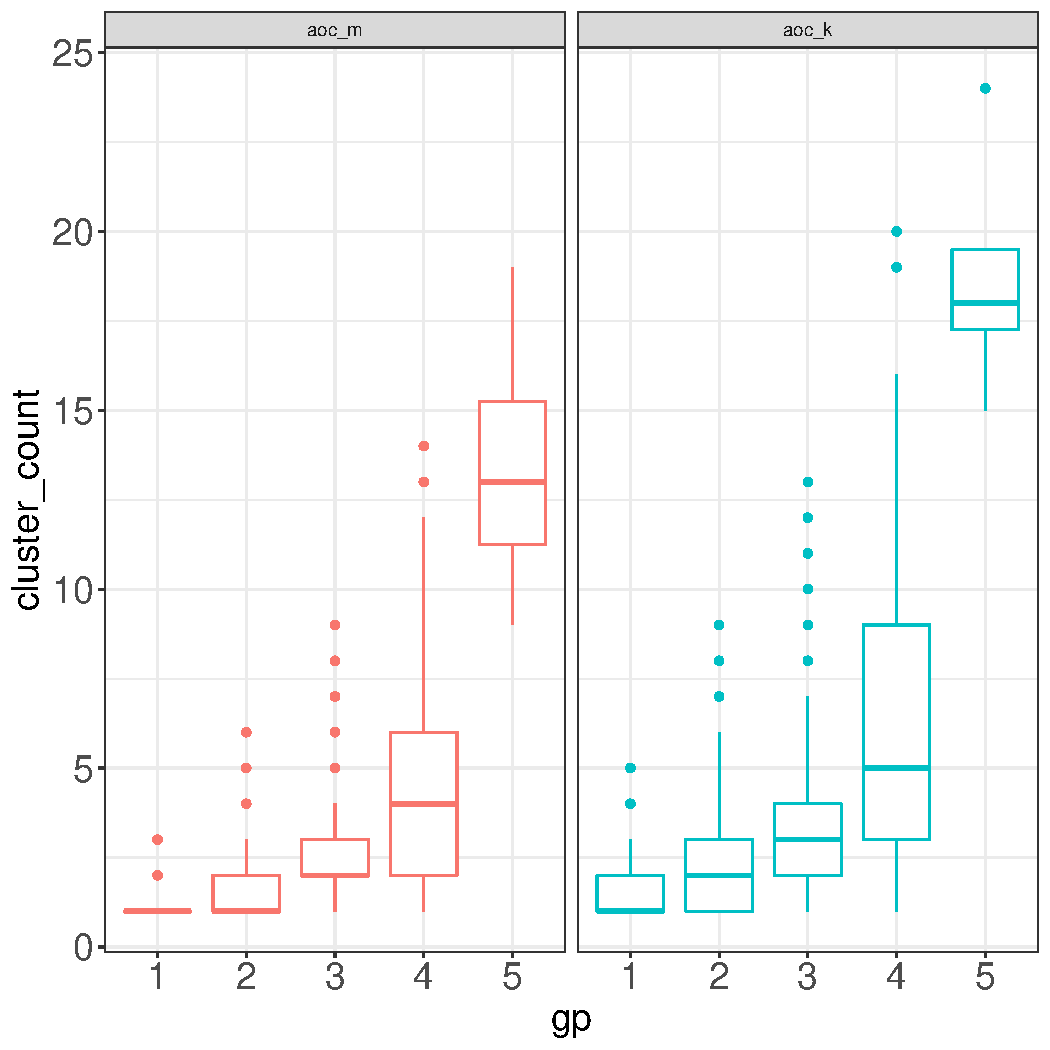
\includegraphics[width=\linewidth]{cluster_group.pdf} 
	 \end{subfigure}
 \hfill
	\begin{subfigure}[t]{0.48\textwidth}
        \centering
        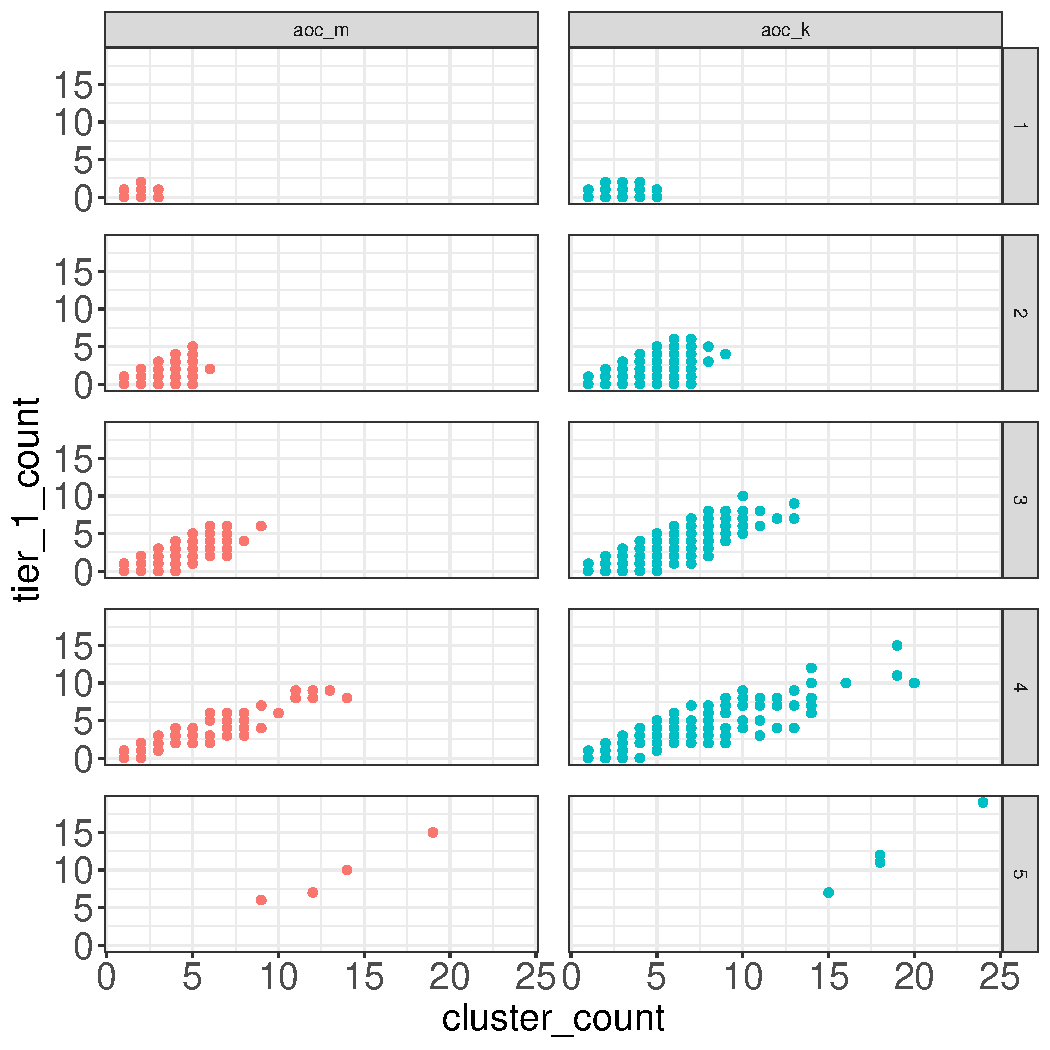
\includegraphics[width=\linewidth]{tier_cluster.pdf} 
    	\end{subfigure}
\captionsetup{width=0.9\textwidth}	
\caption{Cluster and tier assignments by node degree. The subfigure on the left shows the distribution of numbers of clusters each publication belongs to for each group, and the subfigure on the right shows cluster count by tier\_1 membership for each group; each subfigure presents these results for both AOC\_m and AOC\_k. Nodes are partitioned into five groups based on their total in-network degree (in\_degree + out\_degree) with group 1 containing the nodes with the smallest total degree and group 5 with the nodes with the largest total degree. Group 1 has the largest number of observations and group 5 has the smallest. Group Definitons (gp no; class limit; no of nodes): [gp1; $<$100;  272,395], [gp2; 100-999; 254,832], [gp3; 1,000-9,999; 7,773], [gp4; 10,000-99,999; 161], and [gp5; $>$100,000; 4]. }
\label{fig:fig3}
\end{figure}


To ask whether node degree is associated with the number of clusters assigned to, we examined all nodes in the network and compared their in-graph degree to the number of clusters they were assigned, either in AOC\_m or AOC\_k treatment of IKC\_k10 clustering of the CEN (Figure~\ref{fig:fig3}). The first comparison is between clusters produced by AOC\_m (left) and AOC\_k (right), which shows that the number of clusters assignments per node is larger for AOC\_k than for AOC\_m. This is not unexpected since AOC\_m is a more stringent membership criterion. 

We have previously proposed a tier classification for nodes in a cluster, in which Tier 1 refers to the nodes in the top 10th percentile with respect to intra-cluster citations \citep{Chandrasekharan2021}. 
\textcolor{blue}{Check if this is citations or total degree.}
Thus, a Tier 1 node is in the top 10 percent when compared to all other nodes in its cluster when in-degree within the cluster is measured. We observe that nodes assigned to multiple clusters are more likely to have Tier 1 status, that is relatively higher in-degree counts within a cluster (Figure~\ref{fig:fig3}). The Tier 1 count increases for AOC\_k compared to AOC\_m; since cluster size  increases for AOC\_k compared to AOC\_m and Tier 1 contains the top 10\% of the nodes in each cluster, this is also as expected. \textcolor{blue}{Let's discuss this last sentence.}

Turning to AOC\_k specifically, we now consider how in-network degree impacts the total number of clusters each publication is in, and the frequency of Tier 1 membership in these clusters.
The publications are separated  into five groups based on total degree count (Figure~\ref{fig:fig3}).

\textcolor{blue}{I'll take a stab at rewriting this paragraph}.
The first observation is that all the nodes assigned to 14 or more communities have degree at least 10,000, which corresponds to the 99.999th percentile of in-network citations. Only 169 articles have degree of 10,000 or greater in the CEN. 
However the largest number of communities for publications in groups 1 and 2 is 7, group 3 publications appear in at most 9 clusters, group 4 publications appear in up to 13 clusters, 
but group 5 publications appear in up to 25 clusters. In other words, a very high in-graph citation count is necessary  for a publication to appear in many communities. However, the median number of communities for cluster memberships in group 5 is \textcolor{blue}{only KK}, indicating clearly that  an ultra-large citation count seems to be a necessary but not sufficient property for membership in many communities. Furthermore, there are publications from groups 2--4 that also appear in KKK communities, clearly showing that the typical cluster membership count for group 5 (the publications with ultra-large citationcount) can be found as well in publications with much smaller number of citations.

\textcolor{blue}{
Here, again focusing on AOC\_k clustering, we provide some examples
of publications exhibiting a variety of properties.
There are only ZZZ  publications that appear in 14 or more
clusters.  This set includes YYY, and the citation counts for
these publications range from QQQ to WWW.
From Group 5 (the most highly cited nodes), there are some that
appear in a small number of clusters, 
including YYY.
The marker node distribution is also noteworthy, with their
median cluster membership count YYY.
}

\textcolor{blue}{It is also interesting to examine Tier 1 membership.
Some publications are in many clusters but only Tier 1 in a few,
while others are Tier 1 in many of the clusters they belong to.
As examples, YYY.}

\textcolor{blue}{More generally, we see that the number of
clusters a publication belongs to provides a perspective on the publication
that goes beyond its citation count.}


\textcolor{blue}{
We also note that some nodes of high-degree are singletons in IKC(10).
We examine here how many of these remain singletons after
 AOC\_k.
}

\subsection{Experiment 3: Marker node concentrations}

\begin{figure}[H]
	\centering
	 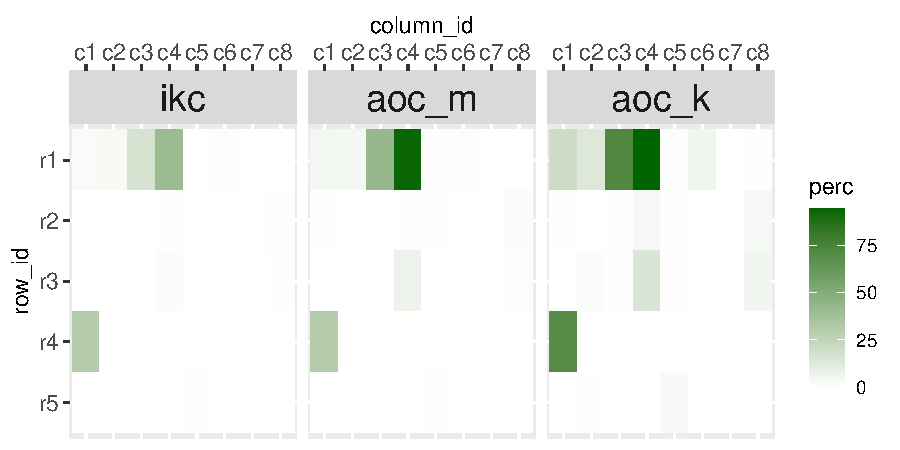
\includegraphics[width=0.7\linewidth]{marker_comps_wide.pdf} 
\caption{NEEDS TO BE REVISED- I have concerns about cluster numbering and the data. Sigh! AOC increases marker node concentration. We show marker node counts in 40 clusters (5 rows with 8 clusters per row) before and after AOC.  Notably, the proportion of 1021 marker nodes in the network increases from 40.7\% in cluster 4 (r1,c4) of IKC clustering to 93.1\% after AOC\_m to 94.6\% after AOC\_k. The proportion of markers in cluster 25 (r4,c1) is the same for IKC and AOC\_m but increases to  69.5\% under the more permissive conditions of AOC\_m. (Data are shown for the 40 clusters with non-zero marker node counts in IKC. Data for all 128 clusters are available in Supplementary Material.)}
\label{fig:marker-node-concentration}
\end{figure}

\clearpage
\begin{table}[H]
\centering
\begin{tabular}{rlcc}
  \hline
 & AOC\_m & no\_change & increase \\ 
  \hline
1 & ikc10 &  33 &  95 \\ 
2 & ikc20 &  10 &  34 \\ 
3 & ikc30 &   8 &  14 \\ 
4 & ikc40 &   3 &   3 \\ 
5 & ikc50 &   1 &   0 \\ 
   \hline
\end{tabular}
\quad
\begin{tabular}{rlcc}
  \hline
 & AOC\_k& no\_change & increase \\ 
  \hline
1 & ikc10 &  17 & 111 \\ 
2 & ikc20 &   2 &  42 \\ 
3 & ikc30 &   4 &  18 \\ 
4 & ikc40 &   2 &   4 \\ 
5 & ikc50 &   1 &   0 \\ 
   \hline
\end{tabular}
\caption{\textcolor{blue}{George, what is this table about? I don't know..}}
\label{tab:tab-unknown}
\end{table}

\subsection{Experiment ??: Examining overlap between clusters}

\begin{figure}[H]
	\centering
	\begin{subfigure}[t]{0.48\textwidth}
	 \centering
	 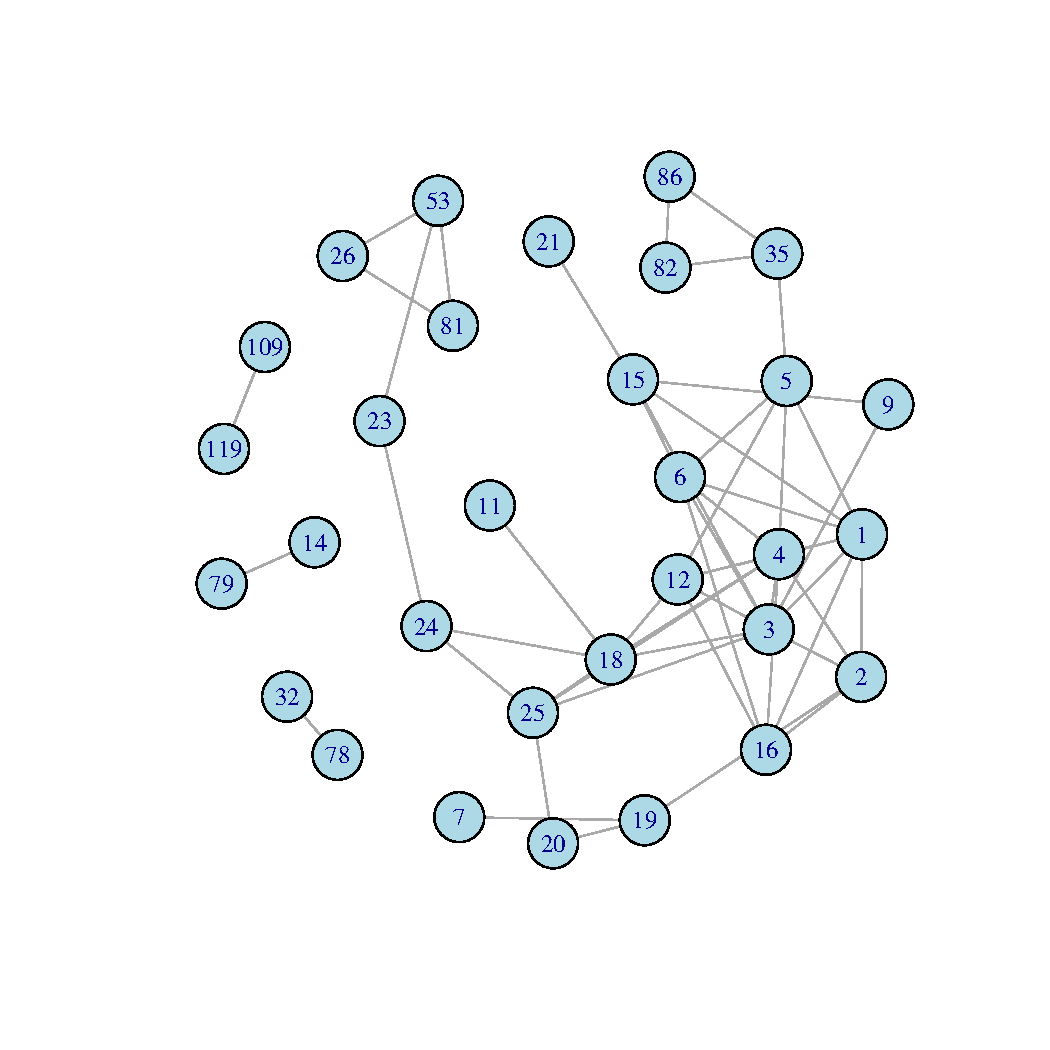
\includegraphics[width=\linewidth]{ikc10_k_pw.pdf} 
	 %\caption{Generic fig2 a caption} \label{fig:2a}
	 \end{subfigure}
 \hfill
	\begin{subfigure}[t]{0.48\textwidth}
        \centering
        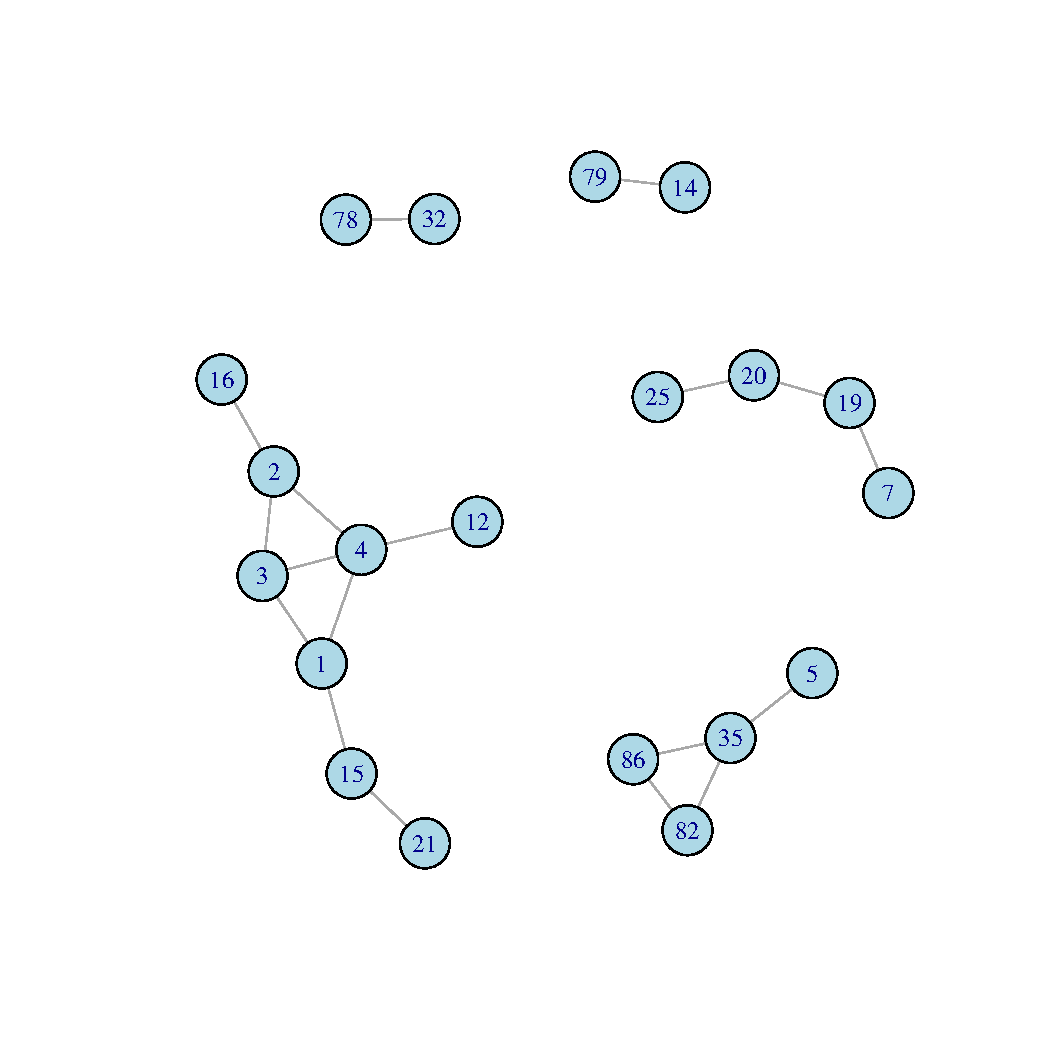
\includegraphics[width=\linewidth]{ikc10_m_pw.pdf} 
        %\caption{Generic fig2 b caption} \label{fig:2b}
    	\end{subfigure}
\caption{NEEDS TO BE REVISED! Overlapping clusters produced by IKC(10)+AOC.  Clusters were generated from CEN data by IKC using $k=10$. These clusters were then enriched through the AOC process enforcing either \emph{k} (left panel) or \emph{mcd} (right panel). 
The clusters produced  by this two-step process are overlapping. We present information about overlap between these clusters using edges and thickness reflecting how much they overlap; only pairs that have overlap Jaccard Coefficient greater  than the median  non-zero overlap Jaccard Coefficient are connected by edges. 
Cluster numbers in both panels retain cluster numbers from the input IKC clustering.}
\label{fig:overlapping}
\end{figure}


\clearpage
\begin{sidewaystable}[h!]
\centering
\resizebox{\textwidth}{!}{
\begin{tabular}{clllllllllll}
  \hline
 no\_clusters & ikc10\_k & ikc10\_m & ikc20\_k & ikc20\_m & ikc30\_k & ikc30\_m & ikc40\_k & ikc40\_m & ikc50\_k & ikc50\_m \\ 
  \hline
1 & 246787 & 442485 & 221728 & 254435 & 85515 & 86806 & 36367 & 36463 & 2004 & 2004 \\ 
2 & 194427 & 78150 & 49195 & 20280 & 2731 & 1487 & 363 & 269 &  &  \\ 
3 & 72367 & 12518 & 4511 & 1057 &  82 &  43 &   4 &   2 &  &  \\ 
4 & 17401 & 1642 & 377 &  98 &  15 &   8 &  &  &  &  \\ 
5 & 3232 & 256 &  61 &  21 &   2 &   1 &  &  &  &  \\ 
6 & 641 &  63 &  19 &   5 &  &  &  &  &  &  \\ 
7 & 168 &  27 &   4 &  &  &  &  &  &  &  \\ 
8 &  64 &   8 &   1 &   1 &  &  &  &  &  &  \\ 
9 &  29 &   5 &   1 &  &  &  &  &  &  &  \\ 
10 &  14 &   1 &   1 &   1 &  &  &  &  &  &  \\ 
11 &   7 &   2 &  &  &  &  &  &  &  &  \\ 
12 &   6 &   3 &  &  &  &  &  &  &  &  \\ 
13 &   5 &   2 &  &  &  &  &  &  &  &  \\ 
14 &   8 &   2 &  &  &  &  &  &  &  &  \\ 
15 &   1 &  &  &  &  &  &  &  &  &  \\ 
16 &   1 &  &  &  &  &  &  &  &  &  \\ 
18 &   2 &  &  &  &  &  &  &  &  &  \\ 
19 &   2 &   1 &  &  &  &  &  &  &  &  \\ 
20 &   2 &  &  &  &  &  &  &  &  &  \\ 
24 &   1 &  &  &  &  &  &  &  &  &  \\ 
   \hline
\end{tabular}}
\caption{Cluster Size Increases After AOC Treatment. The count of clusters that either increase in size (increase) or remain the same size (no\_change) is shown
for either AOC\_m (left) or AOC\_k (right) treatment for five different values of $k$ and where the nodes allowed to be in multiple clusters are those that appear in one non-singleton cluster in IKC(k). 
 For k=50, IKC returns a single cluster; by definition, the cluster does not change after AOC treatment.}
\label{tab:tab2}
\end{sidewaystable}

\clearpage


\subsection{Equilibration Across Cores}

\subsection{Nodes of High Degree}

\subsection{Enforcing MCD}

\subsection{Data}

\section{Conclusions}
\section{Acknowledgments etc.}

\bibliographystyle{apalike}
\bibliography{akhil.bib}
\end{document}
%%%%%%%%%%%%%%%%
%%%%%%%%%%%%%%%%
%%%%%%%%%%%%%%%%
%%%%%%%%%%%%%%%%

